
%TeXstudio produce a LOT of warning yet still compile.

\documentclass[11pt]{beamer} 

\usetheme{metropolis} %https://github.com/matze/mtheme
\metroset{everytitleformat = regular,progressbar=foot} %settings
\mode<presentation>
%\usecolortheme{dove} %dove
% albatross, beaver, beetle, crane, default, dolphin, dove, orchid, rose, seagull, seahorse, whale, wolverine
%dont use  fly, lily,
%http://mirror.ox.ac.uk/sites/ctan.org/macros/latex/contrib/beamer/doc/beameruserguide.pdf
\setbeamercolor{title separator}{fg = UniBlue}
\setbeamercolor{frametitle}{fg = deepBlue, bg=aBlue!70}

\usepackage{booktabs}
\usepackage[scale=2]{ccicons}
\usepackage{pgfplots}
\usepgfplotslibrary{dateplot}
%\usepackage[demo]{graphicx}
\usepackage[font={small,it}]{caption}
\usepackage{subcaption} %throws a lot of errors but compile

%%LOGO
\usepackage{tikz}
\addtobeamertemplate{frametitle}{}{%
\begin{tikzpicture}[remember picture,overlay]
\node[anchor=north east,yshift=2pt] at (current page.north east) {
\includegraphics[height=0.8cm]{./../logo.png}};
\end{tikzpicture}}

%My std preamble for the docs
%\selectlanguage{british}%
\usepackage[british]{babel}
\usepackage{microtype} %better text
\IfFileExists{lmodern.sty}{\usepackage{lmodern}}{} %type 1 vector font
%
\usepackage{lettrine}
\usepackage{listings} %Add list support
\usepackage{colortbl} %colors in TABLES
%\usepackage{tikz,amsmath, amssymb,bm,color}
\usepackage{nicefrac}
\usepackage{lastpage} %get last page

%COLORS
\usepackage{color}
\definecolor{lightgray}{gray}{0.8} %for colortbl
\definecolor{UniBlue}{RGB}{83,121,170}
\definecolor{deepBlue}{HTML}{000066}
\definecolor{blueBgd}{HTML}{99C8FF}
\definecolor{aBlue}{HTML}{1879F7}

%%%%%%%%%%%%%%%%%%%%%%%%%%%%%%%%%%%%%%%%%%%%%%%%%%%%%%%%%%%%%%%%%%
%FOOTNOTES
%nice look after http://www.dedoimedo.com


%%%%%%%%%%%%%%%%%%%%%%%%%%%%%%%%%%%%%%%%%%%%%%%%%%%%%%%%%%%%%%%%%%%
%TABLE SETTINGS
\usepackage{colortbl} %colors in table
\usepackage{rotating} %rotatins within tables
\usepackage{multirow}
\renewcommand{\arraystretch}{1.2} %add padding/spacing
%\usepackage{adjustbox}%rotating and fitting into page
%

\usepackage{booktabs} % To thicken table lines
%define thickness of table lines
\let\mytoprule\toprule
\renewcommand{\toprule}{\mytoprule[0.20em]}
\let\mytoprule\bottomrule
\renewcommand{\bottomrule}{\mytoprule[0.20em]}
\let\mytoprule\midrule
\renewcommand{\midrule}{\mytoprule[0.08em]}

\usepackage{spreadtab} % for simple calculations

%vertically and horizontally centered multicolumn cells with a fixed width. M{width}
%\newcolumntype{M}[1]{>{\centering\hspace{0pt}}m{#1}}
% each spanned cell has the same width. S{width of multicolumn cell}{number of spanned columns}
%\newcolumntype{S}[2]{>{\centering\hspace{0pt}}m{(#1+(2\tabcolsep+\arrayrulewidth)*(1-#2))/#2}}

%%%%%%%%%%%%%%%%%%%%%%%%%%%%%%%%%%%%%%%%%%%%%%%%%%%%%%%%%%%%%%%%%%%
%TikZ
\usepackage{tikz}

\colorlet{red}{red!50}
\colorlet{green}{green!50}
\colorlet{blue}{blue!50}
\definecolor{yellow}{HTML}{FFFF00}
\colorlet{yellow}{yellow!50}
\definecolor{fiolet}{HTML}{7030A0}
\colorlet{fiolet}{fiolet!50}
\colorlet{bgd_main}{black!50}
\colorlet{bgd}{bgd_main!75}
\colorlet{bgd2}{bgd_main!50}
\colorlet{bgd3}{bgd_main!25}
\colorlet{bgd4}{bgd_main!15}

\usetikzlibrary{shapes,arrows,calc,positioning}

%%%%%%%%%%%%%%%%%%%%%%%%%%%%%%%%%%%%%%%%%%%%%%%%%%%%%%%%%%%%%%%%%%%
% Footnotes in Figs
%\rule[raise-height]{width}{thickness}
\newcommand*{\FigFootnote}[1]{
\noindent \begin{flushleft}
\rule[0.2ex]{0.4\columnwidth}{0.5pt}
\par
\footnotesize
#1
\footnotesize
\end{flushleft}
}

%%%%%%%%%%%%%%%%%%%%%%%%%%%%%%%%%%%%%%%%%%%%%%%%%%%%%%%%%%%%%%%%%%%
%MATH, number display
%need to install siunitx, l3kernel,l3packages
\usepackage{siunitx} %this is for units display

\sisetup{per-mode=fraction, tight-spacing = true , fraction-function = \nicefrac, quotient-mode = fraction}% %nicefrac \tfrac
\sisetup{inter-unit-product = \ensuremath { { } \cdot { } } , exponent-product = \cdot }%
\sisetup{input-product=x , output-quotient =  \ensuremath { { } \times{}}} %for 1x2x3
%number grouping(3), std==true %\sisetup{group-digits = decimal} 
\sisetup{group-minimum-digits = 4} %start grouping from 4 digits, in 3 no groups
\sisetup{range-units = single,range-phrase = \,--\,} %2-3C not 2C-3C %, range-phrase = --
\sisetup{separate-uncertainty=true} %2+-1 not 2(1)
\sisetup{prefixes-as-symbols=true } % , scientific-notation = engineering false for 10^-9 ect ect , exp in multiple of 3
\sisetup{range-phrase = \,-\, } % , refo of ranges
%\sisetup{zero-decimal-to-integer, round-mode = places,round-precision = 3}
%\sisetup{add-arc-degree-zero=true , add-arc-minute-zero=true ,add-arc-second-zero=true} %for angle settings

%This is to auto convert ns,ms,us to 10^-xx s
\DeclareSIUnit[scientific-notation = engineering, prefixes-as-symbols=false]{\psec}{\pico\second}
\DeclareSIUnit[scientific-notation = engineering, prefixes-as-symbols=false]{\nsec}{\nano\second} 
\DeclareSIUnit[scientific-notation = engineering, prefixes-as-symbols=false]{\usec}{\micro\second}
\DeclareSIUnit[scientific-notation = engineering, prefixes-as-symbols=false]{\msec}{\milli\second} 

%...AND SOME UNITS
\DeclareSIUnit\dBm{dBm}
\DeclareSIUnit\ppm{ppm} %{\num{1e-6}}%{ppm}
\DeclareSIUnit\yr{yr} %{{361}\day}<-nice nice
\DeclareSIUnit\cy{cycle} %phase cycle
\DeclareSIUnit\epoch{epoch} %GPS/LL epoch
\DeclareSIUnit\inch{"} %inch 
\DeclareSIUnit\wk{week} %week
\DeclareSIUnit\hr{hrs} %hours
\DeclareSIUnit\min{minute} %hours
\DeclareSIUnit\mile{mi}
\DeclareSIUnit\Mcps{Mcps}
\DeclareSIUnit\bit{bit}
\DeclareSIUnit\chip{chip length}
%Other units
\newcommand*{\GBP}[1]{$\SI{#1}[\textsterling]{}$}


%%%%%SHORTHANDS (Standard Sentences)
%\newcommand*{\Myrange}[3]{$\textrm{\SIrange{#1}{#2}{#3}}$}


%how much work per week
\newcommand*{\wkWrk}[1]{$\SI{#1}{\hr\per\wk}$}

%references
\newcommand*{\tabref}[1]{shown in table \ref{#1} on page \pageref{#1}\xspace}
\newcommand*{\vref}[1]{\ref{#1} on page \pageref{#1}\xspace}


%\renewcommand{\baselinestretch}{1.2} %line spacing
%{\setstretch{1.0}\color{blue} text bla bla } for section strech
\renewcommand{\footnotesize}{\scriptsize} %change footnote sizes
\newcommand{\MatlabRef}{\footnote{History of changes at \url{https://github.com/DfAC/TEQCSPEC}.}}
\newcommand{\thisDocRef}{\footnote{History of changes at \url{https://github.com/DfAC/TeachingSlides/}.}}
%\usepackage{lipsum} % for dummy text only

%Grey text
\definecolor{shadecolor}{RGB}{190,190,190}
%\textcolor{shadecolor}{	\item[Ogaja\_Matlab.7z] Matlab script. To be placed on-line after week2.}


%%%%%%%%%%%%%%%%%%%%%%%%%%%%%%%%%%%%%%%%%%%%%%%%%%%%%%%%%%%%%%%%%%%%%%%%%%%%%%
%%%%%%%%%%%%%%%%%%%%%%%%%%%%%%%%%%%%%%%%%%%%%%%%%%%%%%%%%%%%%%%%%%%%%%%%%%%%%%
\title[H24VEP]{H24VEP Project 3}
\subtitle{Bridge Monitoring}

\author{LKB}
\institute{NGI}
\date{\today}

\begin{document}
	
	\begin{frame}
		\titlepage
	\end{frame}
	
	% Uncomment these lines for an automatically generated outline.
	\begin{frame}{Outline}
		\tableofcontents
	\end{frame}
	
\section{Introduction}

\begin{frame}[allowframebreaks]{Project Introduction}

The aim of the project is to characterise bridge movement using precise geodetic sensors. We will monitor Wilford Pedestrian Bridge Monitoring Using GNSS, Robotic Total Station (RTS), IMU and Inclinometer sensors. We will also try to excite the structure to better understand sensors performance and to characterise bridge movement.

To do so we will:

\begin{itemize}
	\item Identify the best layout of the sensors on the bridge;
	\item Decide the details of the trial next week;
	\item Analyse measurements made through different sensors;
	\item Examine the bridge’s response under different excitation types;
	\item Compare and contrast results;
	\item Find the type of excitation which best shows the differences between equipment outputs.
\end{itemize}
\end{frame}

\begin{frame}{Wilford Pedestrian Bridge}
Wilford Pedestrian Bridge is single span suspension bridge. Spans the River Trent; 69 m long and 3.7 m wide.

	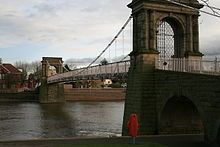
\includegraphics[height=.4\textheight]{pic/Bridge01.jpg}
	\captionof{figure}{Wilford Pedestrian Bridge} %to make images on top of each other
		\centering
	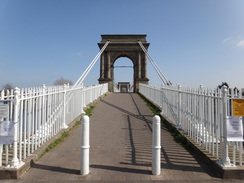
\includegraphics[width=.4\textwidth]{pic/Bridge02.jpg} 
	%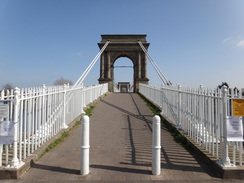
\includegraphics[width=.4\textwidth]{pic/Bridge02.jpg} 

\end{frame}

\begin{frame}{Equipment}
Wilford Pedestrian Bridge is single span suspension bridge. Spans the River Trent; 69 m long and 3.7 m wide.

	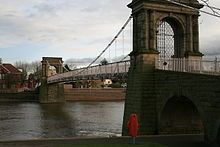
\includegraphics[height=.4\textheight]{pic/Bridge01.jpg}
	\captionof{figure}{Wilford Pedestrian Bridge} %to make images on top of each other
		\centering
	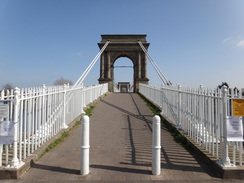
\includegraphics[width=.4\textwidth]{pic/Bridge02.jpg} 
	%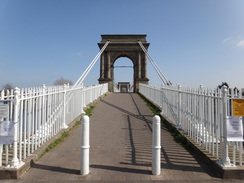
\includegraphics[width=.4\textwidth]{pic/Bridge02.jpg} 

\end{frame}




	\begin{frame}{Workflow}
		I suggest following workflow for your analysis:
		
		\begin{itemize}
			\item Extract QC characteristics from RINEX data using \textit{ teqc +qc +plot data.16o};
			\item Use Matlab script for initial visualisation of results;
			%\item \textcolor{shadecolor}{Examine relevant files and teqc summary file};
			\item Use software to output relevant data into CSV file;
			\item Use Matlab script for initial visualisation of results;
			\item \textbf{Analyse data and draw conclusions.}
			\item \alert{Prepare and present a story about your findings.}
		\end{itemize}
	\end{frame}

%changing settings for this area
{\sisetup{round-mode = places,round-precision = 3} 

\begin{frame}{Point coordinates (truth)}
	\begin{table}
		\centering
		\begin{minipage}[t]{\textwidth}%
			\resizebox{\columnwidth}{!}{%
				\begin{tabular}{lcccc} %{l|c|c|c|c}
					\toprule %\rowcolor{lightgray}
					ID & $E[m]$ & $N[m]$ & Ht Ort [m]\footnote{Geoid undulation is \num{48.523}m} & Notes \\
					\midrule
					JUB7 & \num{454729.5517} & \num{339338.9003} & \num{28.9802} & Open Area\\
					JUB8 & \num{454682.3444} & \num{339523.0937} & \num{27.8030} & Trees\\
					UrbanA & \num{454853.269} & \num{339696.63} & \num{29.89} & MP area for Group A\\
					UrbanB & \num{454858.511} & \num{339697.517} & \num{29.854} & MP area for Group B\\
				\end{tabular}%
			}
			\caption{OSGB coordinates for the Project 1}
		\end{minipage}
	\end{table}
	
\end{frame}
} %{\sisetup{round-mode = places,round-precision = 3} 



\section{Details}



\begin{frame}{Denghui Wang}%{Daily repetition}
	\centering
	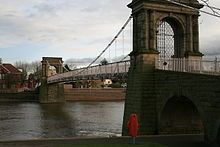
\includegraphics[height=.35\textheight]{pic/Bridge01.jpg}
	\captionof{figure}{Visualisation} %to make images on top of each other
	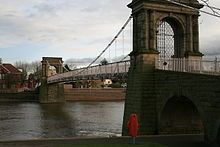
\includegraphics[height=.4\textheight]{pic/Bridge01.jpg} 
	%\captionof{figure}{Example of visualisation}
\end{frame}

\section{Summary}


	\begin{frame}{Summary}
	%For older versions please refer to the GitHub site.
	\end{frame}


%Final slide
\setbeamercolor{background canvas}{bg=blueBgd!60}
\plain{Good luck}



\end{document}
